\section{Analysis}
In this section an analysis of the web interface is explained, using visual aids for the easy understanding of the system functionalities.

\subsection{Database - Paulo Fontes}
For a well constructed database, it has to be consistent, flexible and efficient so no data is lost or repeated when saved. The analysis of the system information given is fundamental for the overview and development of the database structure.

The following use cases are retrieved from the pre-project of the energy hub project. (Project 3 found in appendix):
\paragraph{Use Cases}
	\begin{itemize}
		\item Jan is looking at the web interface for the energy hub. From where he can see the status for each modules connected to it
in a graphically way.
		\item A new energy module is connected to the hub, Jan opens the web interface for the energy hub, he logs into the administrator section of the system
to start, stop or see a more detailed overview of each module.
		\item Jan arrives at the university in the morning and an email was send to him reporting a failure in the green energy system, he login to the administrator web interface, and he can see what the problem might be, and if it's possible to solve it directly on the interface.
	\end{itemize}
From this use cases given by the customer the relevant information for the database design is filtered:
	\begin{itemize}
		\item The status of each module have to be shown.
		\item A detailed overview of each module such as current production (Voltage, Current, Power, etc.), efficiency of the module, etc.
		\item Errors have to be reported to the system administrator / maintainer.
	\end{itemize}
In a deeper analysis of the information system for the power energy hub, some technical data is needed to be stored such as:
	\begin{itemize}
		\item Each module have an unique id, this is similar to the MAC address, in this way, when a module is connected it is possible to check if the module have been connected before, so the data can be stored for the same module instead of instantiate a new module which can generate ambiguous data.
		\item Three types of modules are defined: input, output and bidirectional. This are seen from the power hub point of view where inputs are producers ( solar panels, wind turbine, ... ), output are consumers ( Inverter, 30V output socket ) and bidirectional ( C.A.E.S, batteries, ...).
	\end{itemize}

\paragraph{Data Model}
Data model is a high-level overview of the database structure. At this stage data sets are translated to a logic structure with the relationship between tables.

\begin{figure}[H]
	\begin{centering}
		%\missingfigure{Webserver first page}
		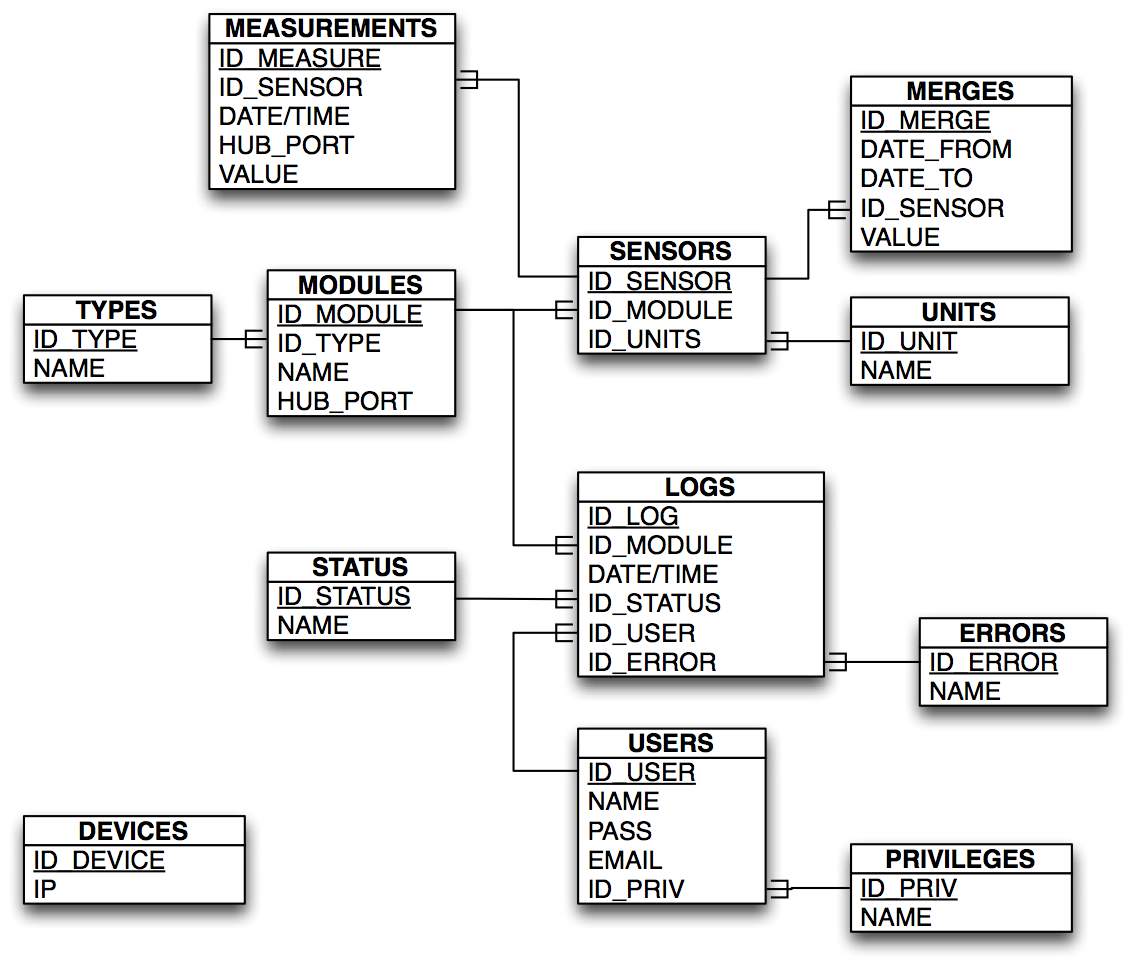
\includegraphics[width=1.0\textwidth]{images/db_datamodel.png}
		\caption{Database relational overview ( Data Model )}
	\end{centering}
\end{figure}

\paragraph{Data sets}
From the system information analysis a basic tabular structure is designed for a better understanding and low level overview of the database, this is called the data set structure.
\\\\

TYPE(ID\_TYPE, NAME);

\begin{table}[H]
\centering
	\begin{tabular}{| p{2cm} | p{10cm} |}
		\hline
		ID\_TYPE & Auto increment integer, a new id number is generated when a different type is needed to the system. \\\hline
		NAME & Describes the type name for example: Input, output, bidirectional, etc.\\\hline
	\end{tabular}
\end{table}

STATUS(ID\_STATUS, NAME);

\begin{table}[H]
\centering
	\begin{tabular}{| p{2cm} | p{10cm} |}
		\hline
		ID\_STATUS & Auto increment integer, a new id number is generated when a different status is needed to the system. \\\hline
		NAME & Describes the status name for example: Running, stopped, warning, etc.\\\hline
	\end{tabular}
\end{table}


MODULES(ID\_MODULE, ID\_TYPE, NAME, HUB\_PORT);

\begin{table}[H]
\centering
	\begin{tabular}{| p{2.2cm} | p{10cm} |}
		\hline
		ID\_MODULE &  Module unique ID, this id as primary key ensures that no module with is repeated in the database.\\\hline
		ID\_TYPE & This is a foreign key for the table type, in this way if some other type of module is needed it can be dynamically added. \\\hline
		NAME & The name of the module for example, Solar Panel, wind turbine, battery. \\\hline
		HUB\_PORT & Actual connected port for this module\\\hline
	\end{tabular}
\end{table}

As a requirement, the database have to store the measurement  from different sensors. This is stored in a the table MEASUREMENTS.

MEASUREMENTS(ID\_MEASURE, ID\_SENSOR, DATE\_TIME, HUB\_PORT, VALUE)

\begin{table}[H]
\centering
	\begin{tabular}{| p{2.2cm} | p{10cm} |}
		\hline
		ID\_MEASURE &  Measurement id, auto increment field.\\\hline
		ID\_SENSOR & This is a foreigner key for the table sensor, this associated the value retrieved to the correspondent sensor. \\\hline
		DATE\_TIME & Date and time of the measurement is saved so it can be plotted or in case of a lower efficiency a detailed history can analysed. \\\hline
		HUB\_PORT & Actual connected port for this module\\\hline
		VALUE & Measurement retrieved by the energy hub.\\\hline
	\end{tabular}
\end{table}

Logs are a simplified method of keeping track about what is happening in the system, this is one of the most fundamental functionalities of the system.

LOGS(ID\_LOG, ID\_MODULE, DATE\_TIME, ID\_STATUS, ID\_USER, ID\_ERROR);

\begin{table}[H]
\centering
	\begin{tabular}{| p{2.2cm} | p{10cm} |}
		\hline
		ID\_LOG & Auto increment integer. A new id number is generated every time a measurement is added. \\\hline
		ID\_MODULE & This is a foreigner key for the table modules, this allow the system to know from which module the measurement corresponds.\\\hline
		DATE\_TIME & Date and time of the log is saved, in case of malfunction it will help with a time line. \\\hline
		ID\_STATUS & The new status of the module that was changed.\\\hline
		ID\_USER & Foreigner key for the table users, this will allow the system to know which user made the change. \\\hline
		ID\_ERROR & Foreigner key for the table error, if any error occurs it will be stored. \\\hline
	\end{tabular}
\end{table}

For error handling situations a table ERRORS is created, in this way the administrator have more control and are able to act in case of some mall function in the system.
\\\\

ERRORS(ID\_ERROR, NAME);

\begin{table}[H]
\centering
	\begin{tabular}{| p{2cm} | p{10cm} |}
		\hline
		ID\_ERROR & Auto increment integer. A new id number is generated when an unknown unit is needed to the system. \\\hline
		NAME & Predefined error description. \\\hline
	\end{tabular}
\end{table}

Measurements are add to the database constantly, which in a non-stop system database size could be a problem, to avoid this situation a MERGES data set is created. This will store an average of values between a time span for each sensor, allowing the customer either to erase the values from the log or export them out from the database.
\\\\

MERGERS(ID\_MERGE, DATE\_FROM, DATE\_TO, ID\_SENSOR, VALUE);

\begin{table}[H]
\centering
	\begin{tabular}{| l | p{10cm} |}
		\hline
		ID\_MERGE & Auto increment integer. A new id number is generated every time an wrap is needed. \\\hline
		ID\_SENSOR & This is a foreigner key for the table sensors, this allow the system to know from which sensor correspond the values .\\\hline
		DATE\_FROM & Date and time of the time span start. \\\hline
		DATE\_TO & Date and time of the time span end. \\\hline
		VALUE & Average measurements value. \\\hline
	\end{tabular}
\end{table}

SENSOR(ID\_SENSOR, ID\_MODULE, ID\_UNITS);

\begin{table}[H]
\centering
	\begin{tabular}{| p{2cm} | p{10cm} |}
		\hline
		ID\_SENSOR & Auto increment integer. A new id number is generated when a different sensor is needed to the system. \\\hline
		ID\_MODULE & This is a foreigner key for the table sensors, this allow the system to know from which module correspond the sensor, being a primary key with the id\_sensor, this way each sensor correspond to only one module .\\\hline
		ID\_UNITS & This is a foreigner key for the table units, which allow the system to know which units the sensor is measuring.\\\hline
	\end{tabular}
\end{table}

UNITS(ID\_UNIT, NAME);

\begin{table}[H]
\centering
	\begin{tabular}{| p{2cm} | p{10cm} |}
		\hline
		ID\_UNIT & Auto increment integer. A new id number is generated when a different unit is needed to the system. \\\hline
		NAME & Describe the unit name for example: A, V, deg ,m/s,etc. (Ampere, Volt, Degrees, Velocity)\\\hline
	\end{tabular}
\end{table}
To increase security, an USERS table is added associated with different PRIVILEGES for different users. A user root is created leaving the system able to manage multiple users with different privileges if needed.
\\

USERS(ID\_USER, NAME, PASS, EMAIL, ID\_PRIV);

\begin{table}[H]
\centering
	\begin{tabular}{| p{2cm} | p{10cm} |}
		\hline
		ID\_USER & Auto increment integer. A new id number is generated when a different privilege is needed to the system. \\\hline
		NAME & Username credential. \\\hline
		PASS & User password (Not encrypted in this version). \\\hline
		EMAIL & Email to which warnings are send. \\\hline
		ID\_PRIV & Foreigner key for the table privileges. \\\hline
	\end{tabular}
\end{table}

PRIVILEGES(ID\_PRIV, NAME);

\begin{table}[H]
\centering
	\begin{tabular}{| p{2cm} | p{10cm} |}
		\hline
		ID\_UNIT & Auto increment integer, a new id number is generated when a different privilege is needed to the system. \\\hline
		NAME & Describe the user privileges. \\\hline
	\end{tabular}
\end{table}
For the communication process between the web interface and the energy hub, the ip address of the device need to be always accessible this way a table DEVICES is created in which the last known IP address of the device is stored.
\\\\

DEVICES(ID\_DEVICE, IP);

\begin{table}[H]
\centering
	\begin{tabular}{| p{2cm} | p{10cm} |}
		\hline
		ID\_DEVICE & Auto increment integer, a new id number is generated when a different ip added. \\\hline
		IP & IP address of the device. \\\hline
	\end{tabular}
\end{table}

At this point, in an abstract way, the database can initialise a new module or identify if the module where connected before, change the status for each module and add new measurements for each sensor.

\subsection{File Structure - Theis Christensen }
The file structure defines how files are grouped on a system, in a web server architecture the files are stored in the root directory defined by the web server (Apache) configuration. This section describes the analysis of a file structure that allows the scalability of the system.

\paragraph{Overview}
New modules are added are removed from the energy hub as needed. Some modules have different functionalities that have to be taken in consideration when defining the file structure.

In the root directory of the web server the main page is the entrance to the web interface navigation, from here the user can see the modules connected to the energy hub, and some values about the system such as the efficiency of the green energy system. From the main page the user is able to navigate to the different modules page.

To keep the system dynamic, and flexible the modules page are included inside a predefined layout using PHP. This will keep the graphic layout and navigation system in each page consistent and further improvements for the user experience can be made.

The proposed file structure can be seen bellow:
\begin{figure}[H]
	\begin{centering}
		%\missingfigure{Webserver first page}
		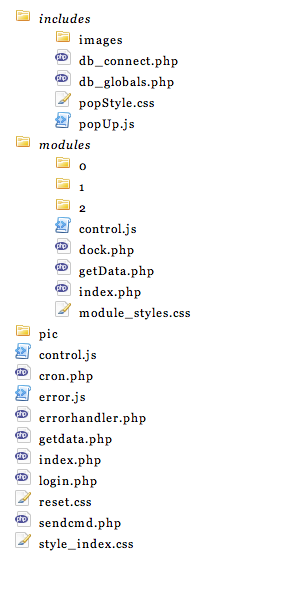
\includegraphics[width=0.3\textwidth]{images/file_structure.png}
		\caption{Proposed File structure}
	\end{centering}
\end{figure}

A short description for each script listed above can be seen in this list:
\begin{itemize}
	\item includes/images/ - Contains images related with the system functionalities.
	\item includes/db\_connect.php - Handle the connection to the MySQL database.
	\item includes/db\_globals.php - Includes all the global variables with the credentials for the database.
	\item includes/popStyle.css - Popup login style definition.
	\item includes/popUp.js - Client side script to handle the user login.
	\item modules/[0-2] - Modules pages, the numbers are associated with the modules ids, being 0 the hub, 1 the battery and 2 the photovoltaic panels.
	\item modules/control.js - Client side script, makes background requests to a PHP script, this script is part of the user experience optimization.
	\item modules/dock.php - PHP script contains the navigation system for the web interface.
	\item modules/getdata.php - PHP script called in background by the client side script running recursively control.js, this script retrieves the system status and data form database in real time, is part of the user experience optimization.
	\item modules/index.php - This page includes each module page structure.
	\item modules/module\_styles.css - Graphical layout definition.
	\item control.js - Client side script, makes background requests to a PHP script and handle the connections of new modules, this script is part of the user experience optimization.
	\item cron.php  - Cron jobs are running by the server in a predefined time, in this case the cron.php at the web server root will point to the cron jobs inside each module folder.
	\item error.js - Client side script, make background requests to a PHP script part of the error handling system.
	\item errorhandler.php - PHP script called in background by the client side script running recursively, is part of the error handling system.
	\item getdata.php - PHP script called in background by the client side script running recursively control.js, this script retrieves the modules connected to the system in real time. Is part of the user experience optimization.
	\item index.php - First page of the web interface.
	\item login.php  - This PHP script is called in background by the pop up login client side script.
	\item reset.css - Layout definition of the web interface.
	\item sendcmd.php - Webservice to send commands to the desired module/enegy hub.
	\item style\_index.css - Layout definition of the web interface.
\end{itemize}

Due to the size of such system and the few time for the development, the project was scaled down so a high fidelity prototype where the system to be can be implemented and the main functionalities of the system tested.

\subsection{Communication - Dennis Madsen}
The web interface is the connection between the user and the system, in this interface the user have to be able to see the data retrieved by the modules and at the same time be able to send commands to the energy hub/modules to do predefined tasks.

To retrieve the measurements from the modules, an application running at the energy hub translates the data retrieved from the module through PLC to a URL request at the web server. In the server side a script is implemented to translate this request to a SQL query which then saves the measurement in the database. It is important to define which data the server side script will expect from the energy hub request. Since each module can have more than one sensor it is important to retrieve the sensor id, the measured value and the energy hub port that this module is connected to.

The communication between the energy hub and the web server is not exclusive for adding new measurements to the database, the communication can also be used to update the database regarding the status of the modules in case of new connection, disconnection, malfunction or if it is stopped for security reasons. The data is saved in the table logs and shown to the user.

\begin{figure}[H]
	\begin{centering}
		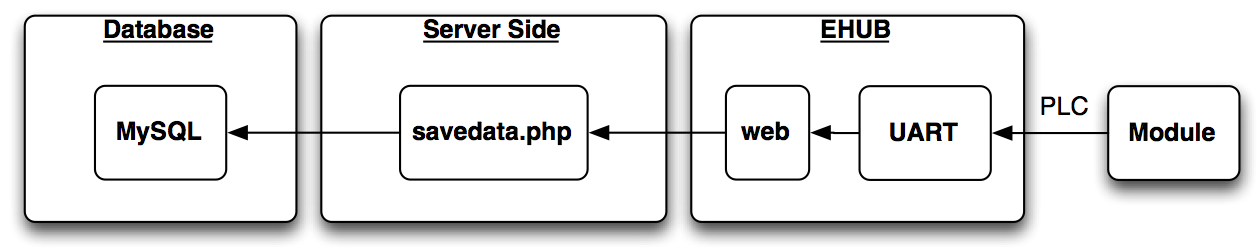
\includegraphics[width=1\textwidth]{images/savedata.png}
		\caption{Save data to the database}
	\end{centering}
\end{figure}

As defined in the Project 3 (see appendix) requirements the system have to give the possibility for the administrator to control the modules and the energy hub. As such the web server have to stablish a connection to the system so commands can be send. A feedback of success or failure is always given to the user since the command to be send can be of great importance for the well function of the system.

The flow of communication from the user until the final destination in this case the module or the energy hub.
\begin{figure}[H]
	\begin{centering}
		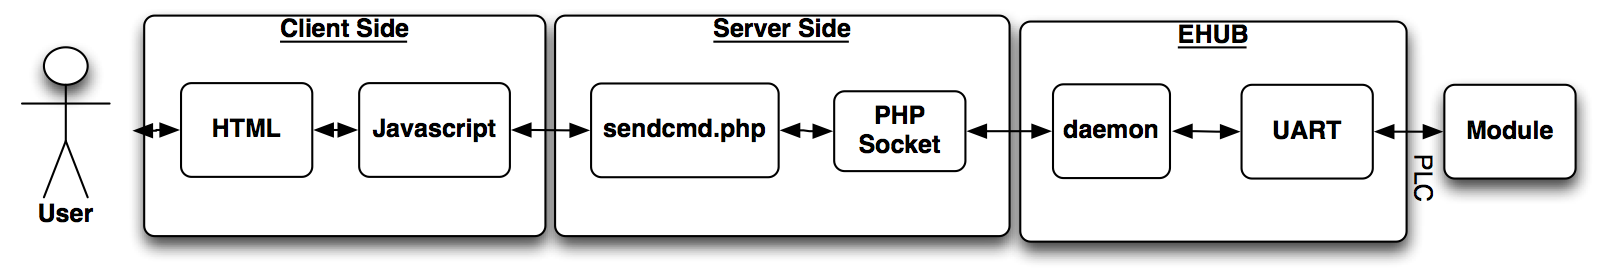
\includegraphics[width=1\textwidth]{images/sendcmd.png}
		\caption{Send a command to a module or energy hub}
	\end{centering}
\end{figure}

A background application running at the energy hub, ensures that after a reboot, the IP address assigned by DHCP to the energy hub is saved in the database, this way commands can be send through the web interface. The system becomes more flexible in case of internal network changes.
\begin{figure}[H]
	\begin{centering}
		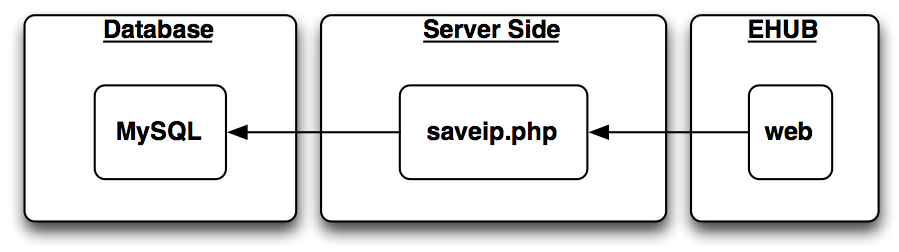
\includegraphics[width=0.8\textwidth]{images/saveip.png}
		\caption{Save the IP address of the Embedded device}
	\end{centering}
\end{figure}

\subsection{Error Handling - Paulo Fontes}
The web server have to be able to handle errors such the lost of communication with the energy hub or database connection problems. For a reliable system, a script running on the client side using JavaScript have to be implemented, this way the web interface can recursively test the communication to the energy hub and database.

Is necessary to define the web interface response for both situations database and energy hub connection lost. If the connection is lost to the device the user is able to see the data stored in the database, so the system is not blocked, but a warning is shown to the user/administrator, do the correspondent debug can be done. In case the connection to the database is lost, the user interface is blocked with an warning, the energy hub will continue working, since it doesn't affected the correct work of the system to route the energy, in this situation all the data retrieved by the modules will be lost.

Since a script is running recursively at the client side, when the communications are re-establish to the energy hub or database the user will be able to use the system normally, this is a great improvement in the user experience and functionalities as an web application.
